\chapter{Modeling} \label{chap:modeling}
In order to evaluate the possibilities of applying Reinforcement Learning in AUV control simulations will be conducted using the \textbf{BlueROV2} by \textit{BlueRobitcs} \cite{blue}. The BlueROV2 has a 6-thruster vectored configuration, open-source electronics and software, and works well for inspections, research, and adventuring. The simulation model does not include the BlueROVs' tether, which connects the vehicle to i.e a surface vessel, which means that the vehicle is \textit{assumed to perform as an AUV in simulation}. 
\begin{figure}[H]
    \centering
    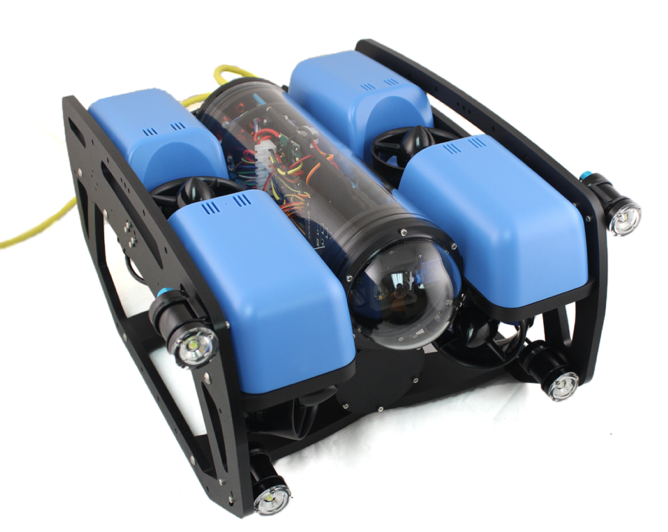
\includegraphics[width=0.7\textwidth]{images/chap4/bluerov2.png}
    \caption{BlueROV2 by BlueRobotics \cite{blue}}
    \label{fig:bluerov2}
\end{figure}
\section{Reference frames}
\begin{figure}[H]
    \centering
    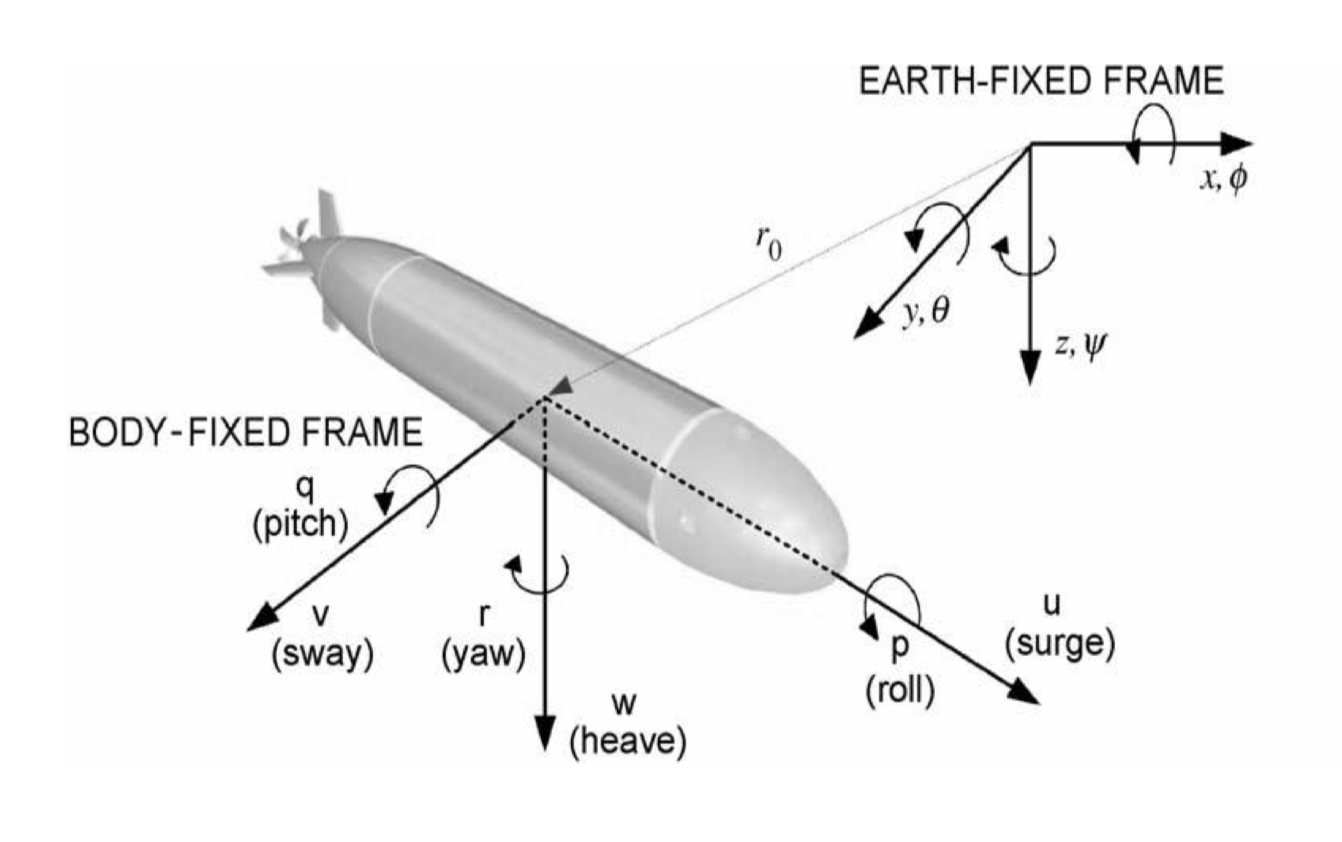
\includegraphics[width=0.7\textwidth]{images/chap4/reference_frames.png}
    \caption{Body fixed and earth fixed reference frame}
    \label{fig:reference_frame}
\end{figure}
In figure \ref{fig:reference_frame} the BlueROV2s' 6 degrees of freedom (DOFs) in the \textbf{Body-fixed} and \textbf{Earth-fixed} reference frame are illustrated. Here the \textbf{North-East-Down} (NED) reference frame will be used as the earth-fixed reference frame. When analysing motion in 6 DOFs it is convenient to define motion in different reference, or coordinate, frames. The reference frames are given by
\begin{itemize}
    \item \textit{NED} is defined as a coordinate system $\{n\} = (x_{n},y_{n},z_{n})$ with origin $o_{n}$ relative to the Earth's reference ellipsoid, commonly defined as the tangent plane to the surface of the Earth moving with the vessel \cite{Fossen}. Here, the $x_{n}$ axis points towards true North, the $y_{n}$ axis points towards the true East and the $z_{n}$ axis points downwards normal to the surface. 
    \item \textit{Body} is defined as a coordinate system $\{b\} = (x_{b},y_{b},z_{b})$ with origin $o_{b}$ centred at the vessels centre of mass, and moving with the body. Here, the $x_{b}$ axis is directed from aft to fore, the $y_{b}$ transverse axis is directed towards starboard and the $z_{b}$ normal axis directed from top to bottom. 
\end{itemize}
The notations in figure \ref{fig:reference_frame} are defined according to SNAME (1950) \cite{Fossen}, which is given in figure \ref{fig:sname}. The SNAME notation will be used throughout this report. 
\begin{figure}[H]
    \centering
    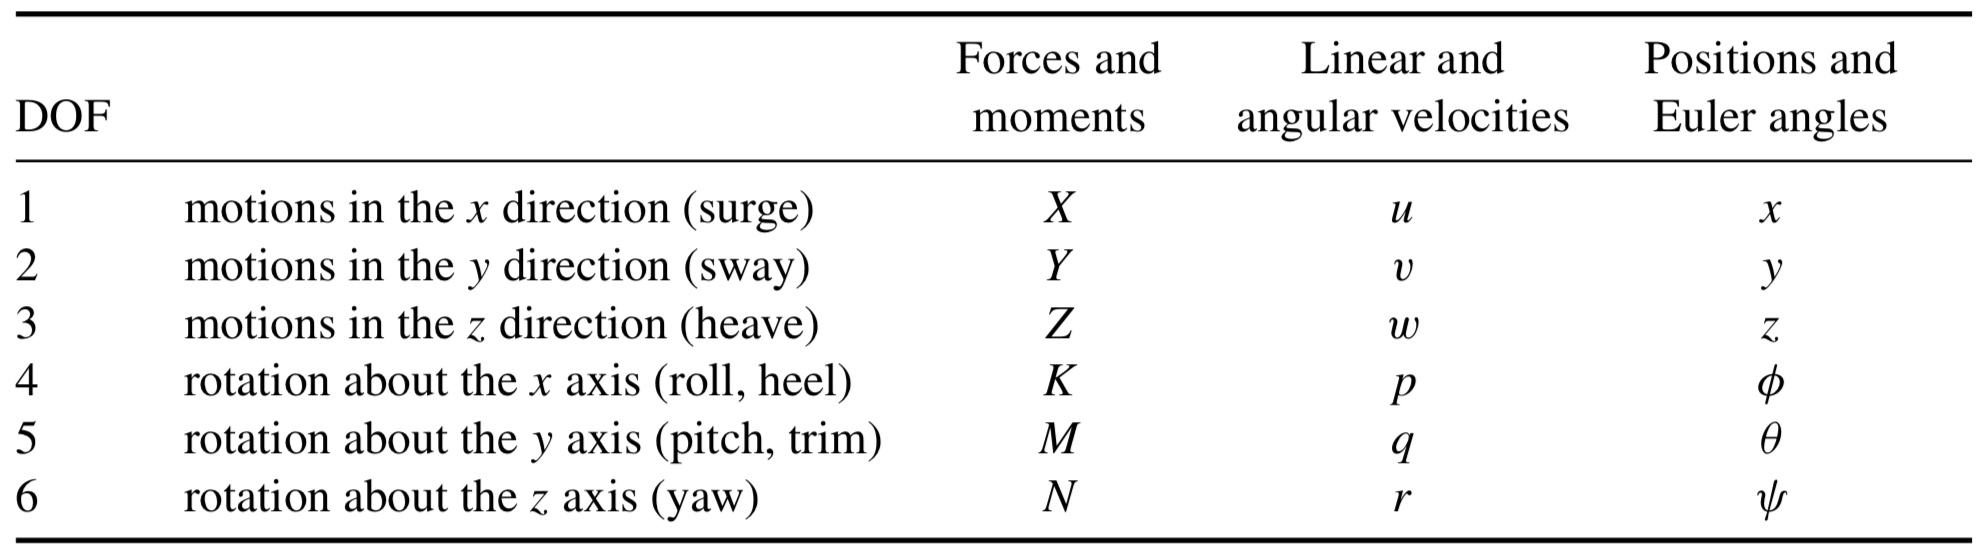
\includegraphics[width=\textwidth]{images/chap4/SNAME.png}
    \caption{The notation of SNAME (1950) for marine vessels}
    \label{fig:sname}
\end{figure}
When dealing with multiple frames it is necessary to \textit{transform} between them, such that any parameter can be expressed in all frames. This is done through a \textit{transformation matrix}. For the BlueROV2 the linear and angular velocities, given in figure \ref{fig:sname}, are defined in the (Body) reference frame. From \textit{Fossen} \cite{Fossen} the \textit{Euler angles}, roll ($\phi$), pitch ($\theta$) and yaw ($\psi$), can be used to decompose the velocity vector $\textbf{v}_{b/n}^{b}$ in the (NED) reference frame. This is given by
\begin{equation}
    \mathbf{v}_{b/n}^{n} = \mathbf{R}_{b}^{n}(\Theta_{nb})\mathbf{v}_{b/n}^{b}
\end{equation}
where the rotation matrix from (Body) to (NED) is given by
\begin{equation}
    \mathbf{R}_{b}^{n}(\Theta_{nb}) = \begin{bmatrix}
    c\psi c\theta & -s\psi c \phi + c\phi s\theta s\phi & s\psi s\phi + c\psi c\phi s\theta \\ s\psi c\theta & c\phi c\phi + s\phi s\theta s\psi & -c\psi s\phi + s\theta s\psi c\phi \\ -s\theta & c\theta s\phi & c\theta c\phi 
    \end{bmatrix}
\end{equation}
where $c=cos$ and $s=sin$.
\section{Dynamic Model of Underwater Vehicles}
From \textit{Fossen} \cite{Fossen} the underwater dynamic equation of motions can be expressed as
\begin{align}
    M\Dot{v}+C(v)v+D(v)v+g(\mu)+\delta & = \tau \\
    \longrightarrow (M_{RB}+M_{A})\Dot{v}+(C_{RB}(v)+C_{A}(v))v+(D_{L}+D_{Q})v + g(\mu)+\delta & = \tau 
    \label{eq:motion}
\end{align}
For simplicity the external forces, in example environmental forces $\tau_{env}$, are here neglected. $\tau$ is therefore the forced applied by the controller, while $\delta$ is a model uncertainty vector. The terms in equation \ref{eq:motion} are defined in the following sections, and their values are given in Appendix A. 
\subsection{Mass matrix}
The Mass matrix consist of \textit{rigid-body} terms and \textit{hydrodynamic} terms. The hydrodynamic terms are due to \textit{added mass}, which is mass created by the acceleration of the surrounding water when a vehicle is moving through a stationary fluid \cite{Fossen}. 
\begin{align}
    \textbf{M}_{RB} & = \begin{bmatrix}
                m*I_{3x3} & 0_{3x3}\\
                0_{3x3} & I_{g}
                \end{bmatrix} \\
    \mathbf{I}_{g} & = \begin{bmatrix}
                I_{x} & -I_{xy} & -I_{xz} \\
                I_{yx} & I_{y} & -I_{yz} \\
                -I_{zx} & -I_{zy} & I_{z}
                \end{bmatrix} \\
    \textbf{M}_{A} & = \begin{bmatrix}
                X_{\Dot{u}} & X_{\Dot{v}} & X_{\Dot{\omega}} & X_{\Dot{p}} & X_{\Dot{q}} & X_{\Dot{r}} \\
                Y_{\Dot{u}} & Y_{\Dot{v}} & Y_{\Dot{\omega}} & Y_{\Dot{p}} & Y_{\Dot{q}} & Y_{\Dot{r}} \\
                Z_{\Dot{u}} & Z_{\Dot{v}} & Z_{\Dot{\omega}} & Z_{\Dot{p}} & Z_{\Dot{q}} & Z_{\Dot{r}} \\
                K_{\Dot{u}} & K_{\Dot{v}} & K_{\Dot{\omega}} & K_{\Dot{p}} & K_{\Dot{q}} & K_{\Dot{r}} \\
                M_{\Dot{u}} & M_{\Dot{v}} & M_{\Dot{\omega}} & M_{\Dot{p}} & M_{\Dot{q}} & M_{\Dot{r}} \\
                N_{\Dot{u}} & N_{\Dot{v}} & N_{\Dot{\omega}} & N_{\Dot{p}} & N_{\Dot{q}} & N_{\Dot{r}} \\
                \end{bmatrix} \\
\end{align}
where \textbf{m} denotes the total mass of the vehicle, and \textbf{I$_{x}$, I$_{y}$, I$_{z}$} represents the moment of inertia about the body axis. Because of symmetry, the products of inertia, here represented on the off-diagonal, will have the form \textbf{I$_{xy}$} = \textbf{I$_{yx}$}, \textbf{I$_{yz}$} = \textbf{I$_{zy}$} and \textbf{I$_{zx}$} = \textbf{I$_{xz}$}. The added mass matrix consist of hydrodynamic derivatives, which is given by
\begin{equation}
N_{\Dot{k}} = \frac{\partial N}{\partial \Dot{k}}
\end{equation}
where N = ($X, Y, Z, K, M, N$) and k = ($u, v, \omega, p, q, r$). In example, $X_{\Dot{u}}$ represent the added mass force coefficient in surge due to an acceleration in surge.
\subsection{Coriolis and Centripetal force matrices}
The Coriolis-Centripetal matrix will also consist of a rigid-body and hydrostatic term. From Fossen \cite{Fossen} the rigid-body Coriolis-Centripetal matrix can be found by defining $\textbf{M}_{RB}$ as
\begin{equation}
    \mathbf{M}_{RB} = \mathbf{M}_{RB}^{T} = \begin{bmatrix}
    \mathbf{M}_{11} & \mathbf{M}_{12} \\
    \mathbf{M}_{21} & \mathbf{M}_{22}
    \end{bmatrix} > 0
\end{equation}
where $\textbf{M}_{21}=\textbf{M}_{12}^T$. $\mathbf{C}_{RB}$ is then found by
\begin{equation}
    \mathbf{C}_{RB}(\mathbf{\nu}) = \begin{bmatrix}
    0_{3x3} & -S(M_{11}\nu_{1}+M_{12}\nu_{2}) \\
    -S(M_{11}\nu_{1}+M_{12}\nu_{2}) & -S(M_{21}\nu_{1}+M_{22}\nu_{2})
    \end{bmatrix}
\end{equation}
where $\nu_{1} := v_{b/n}^{b} = [u, v, \omega]^{T}, \nu_{2} := \omega_{b/n}^{b}=[p, q, r]^{T}$ and $S$ is the cross-product operator. The hydrodynamic Coriolis-Centripetal matrix can be found in the same way, by using $\textbf{M}_{A}$. This yields
\begin{align}
    \mathbf{M}_{A} & = \mathbf{M}_{A}^{T} = \begin{bmatrix}
    \mathbf{A}_{11} & \mathbf{A}_{12} \\
    \mathbf{A}_{21} & \mathbf{A}_{22}
    \end{bmatrix} > 0 \\
    \mathbf{C}_{A}(\mathbf{\nu}) & = \begin{bmatrix}
    0_{3x3} & -S(A_{11}\nu_{1}+A_{12}\nu_{2}) \\
    -S(A_{11}\nu_{1}+A_{12}\nu_{2}) & -S(A_{21}\nu_{1}+A_{22}\nu_{2})
    \end{bmatrix}
\end{align}
\subsection{Damping matrices}
As stated previously the environmental forces are neglected in equation \ref{eq:motion}, which means that skin friction and vortex shedding will dominate the damping term. This leads to the simplified hydrodynamic damping terms in equation \ref{eq:damp} and \ref{eq:damp1}.
\begin{align}
    \mathbf{D}_{L} & = -\begin{bmatrix}
                X_{u} & 0 & 0 & 0 & 0 & 0\\
                0 & Y_{v} & 0 & 0 & 0 & 0 \\
                0 & 0 & Z_{\omega} & 0 & 0 & 0 \\
                0 & 0 & 0 & 0 & K_{p} & 0 & 0 \\
                0 & 0 & 0 & 0 & 0 & M_{q} & 0 \\
                0 & 0 & 0 & 0 & 0 & 0 & N_{r} 
                \label{eq:damp}
                \end{bmatrix} \\
    \mathbf{D}_{Q} & = -\begin{bmatrix}
                X_{u|u|}|u| & 0 & 0 & 0 & 0 & 0\\
                0 & Y_{v|v|}|v| & 0 & 0 & 0 & 0\\
                0 & 0 & Z_{\omega|\omega|}|\omega| & 0 & 0 & 0\\
                0 & 0 & 0 & K_{p|p|}|p| & 0 & 0 \\
                0 & 0 & 0 & 0 & M_{q|q|}|q| & 0 \\
                0 & 0 & 0 & 0 & 0 & N_{r|r|}|r|
                \label{eq:damp1}
                \end{bmatrix}|\mathbf{v}| \\
\end{align}
\subsection{Hydrostatic terms}
The hydrostatic matrix, expressed as $g(\mu)$ in equation \ref{eq:motion}, accounts for the \textit{restoring forces}, which is defined as the relationship between weight, W, and buoyancy, B. By assuming that the vehicle is \textit{neutrally buoyant} it will satisfy $W = B$, and by further assuming that the \textit{centre of gravity} (COG) and the \textit{centre of buoyancy} (COB) are located vertically on the $z$ axis, the hydrostatic matrix can be defined as in \cite{Fossen}
\begin{equation}
    g(\mu) = [0, 0, 0, \Bar{BG}_{z} W cos(\phi)sin(\phi), \Bar{BG}_{z} W sin(\theta), 0]^{T}
\end{equation}
where $\Bar{BG}_{z}=z_{g}-z_{b}$, with $z_{g}$ being the $z$ component in COG, and $z_{b}$ being the $z$ component in COB, and $\mu = [N, E, D, \phi, \theta, \psi]$ in the (NED) and (Body) reference frames. 
\chapter{Method} \label{chap:method}
\section{Controller implementation for the BlueROV2}
The \textbf{BlueROV2} has 13 states, which are defined hereafter as
\begin{itemize}
    \item 3 \textit{position} states defined in the (NED) frame as [$x$, $y$, $z$]
    \item 4 \textit{orientation} states defined in the (NED) frame as the quaternions [$\epsilon_{1}$, $\epsilon_{2}$, $\epsilon_{3}$, $\eta$]
    \item 3 \textit{linear velocity} states defined in the (Body) frame as [$u$, $v$, $w$]
    \item 3 \textit{angular velocity} states defined in the (Body) frame as [$p$, $q$, $r$]
\end{itemize}
The orientation states are defined as \textit{quaternions} in order to resolve the issue connected to singularity in $\theta = \pm 90 \deg$ when using \textit{Euler angles}. However, in order for the controller to use these states they need to be transformed into Euler angles. The singularity wont be an issue when doing this, since the transformation don't affect the model measurements. From (eq. 2.58) in Fossen \cite{Fossen} it is given that the \textit{rotation matrix} from (BODY) to (NED) for the quaternions is defined as
\begin{equation}
    \mathbf{R}_{b}^{n}(\mathbf{q}) = 
    \begin{bmatrix}
    1 - 2(\epsilon_{2}^{2}+\epsilon_{3}^{2}) & 2(\epsilon_{1}\epsilon_{2}-\epsilon_{3}\eta) & 2(\epsilon_{1}\epsilon_{3}+\epsilon_{2}\eta) \\
    2(\epsilon_{1}\epsilon_{2}+\epsilon_{3}\eta) & 1 - 2(\epsilon_{1}^{2}+\epsilon_{3}^{2}) & 2(\epsilon_{2}\epsilon_{3}-\epsilon_{1}\eta) \\
    2(\epsilon_{1}\epsilon_{3}-\epsilon_{2}\eta) & 2(\epsilon_{2}\epsilon_{3}+\epsilon_{1}\eta) & 1 - 2(\epsilon_{1}^{2}+\epsilon_{2}^{2})
    \end{bmatrix}
\end{equation}
Furthermore, from (eq. 2.76) it is given that
\begin{equation}
    \mathbf{R}_{b}^{n}(\Theta_{nb}) := \mathbf{R}_{b}^{n}(\mathbf{q})
\end{equation}
which gives the relationship between the Euler angles, $\phi$, $\theta$ and $\psi$, and the quaternions defined as 
\begin{equation}
    \begin{bmatrix}
    c\psi c\theta & -s\psi c \phi + c\phi s\theta s\phi & s\psi s\phi + c\psi c\phi s\theta \\ s\psi c\theta & c\phi c\phi + s\phi s\theta s\psi & -c\psi s\phi + s\theta s\psi c\phi \\ -s\theta & c\theta s\phi & c\theta c\phi 
    \end{bmatrix}
    = \begin{bmatrix}
    R_{11} & R_{12} & R_{13} \\ R_{21} & R_{22} & R_{23} \\ R_{31} & R_{32} & R_{33}
    \end{bmatrix}
\end{equation}
here $c = cos$ and $s = sin$. This results in the following Euler angles, which is used in the controller
\begin{align}
    \phi & = atan2(R_{32}, R_{33}) = atan2(2(\epsilon_{2}\epsilon_{3}+\epsilon_{1}\eta), 1 - 2(\epsilon_{1}^{2}+\epsilon_{2}^{2})) \\
    \theta & = -sin^{-1}(R_{31}) = -sin^{-1}(2(\epsilon_{1}\epsilon_{3}-\epsilon_{2}\eta)) \\
    \psi & = atan2(R_{21}, R_{11}) = atan2(2(\epsilon_{1}\epsilon_{2}+\epsilon_{3}\eta), 1 - 2(\epsilon_{2}^{2}+\epsilon_{3}^{2}))
\end{align}
$\phi$ and $\theta$ defines roll and pitch, respectively. In order to simplify the implementation of a controller based on Reinforcement Learning it is convenient to not include these two in the algorithm. The reason for this is that the overall goal is to accomplish Station Keeping, and these two states are not as "important" as the rotation about the z-axis, $\psi$. To further simplify the problem the position in $z$ is also neglected, since constant depth is assumed.\\\\
Although these three states, $\phi$, $\theta$ and $z$, are not accounted for by the Reinforcement Learning algorithm, meaning that the algorithm do \textit{not} produce thrust input for these direction/orientations, their states will \textbf{affect} the behaviour of the vehicle. In order to resolve this a \textit{classical} control algorithm will first be implemented, to make these three states stable on their own. Then the Reinforcement Learning algorithm will be implemented for controlling the resulting states.

\subsection{Implementation of PD algorithm}
As mentioned in chapter \ref{chap:station-keeping}, the PID algorithm is a common method for control, but in most cases only using a PD algorithm will be sufficient. In order to accomplish Station Keeping of the AUV the PD algorithm should adjust thrust in the $z$ direction as well as the $\phi$ and $\theta$ rotations. The PD algorithm is thereby given by
\begin{align}
    \tau & = K_{p}e(t) + K_{d}\frac{d(t)}{dt} \\
    \longrightarrow
    \begin{bmatrix}
    \tau_{z}(t) \\ \tau_{\phi}(t) \\ \tau_{\theta}(t) 
    \end{bmatrix}
    & = K_{p} \begin{bmatrix}
    e(t)_{z} \\ e(t)_{\phi} \\ e(t)_{\theta} 
    \end{bmatrix}
    + K_{d} \begin{bmatrix}
    \omega(t) \\ p(t) \\ q(t)
    \end{bmatrix}
\end{align}
\subsection{Implementation of DDPG algorithm}
As mentioned in chapter \ref{chap:station-keeping} the DDPG is a policy-gradient algorithm, which uses a stochastic behaviour policy for good exploration, but estimates a deterministic target policy, which is easy to learn. In order to implement this there will be used two \textbf{neural networks}, a \textit{control} neural network (actor) and an \textit{evaluation} neural network (critic), based on the experiments done by (Yu, Runsheng., et al.) \cite{Yu}.\\\\
In order to define the neural networks the equation of motions for underwater vehicles, defined in equation \ref{eq:motion}, is used. By assuming the roll rotation ($\phi$) and the pitch direction ($\theta$) small, the rotation matrix from (Body) to (NED) can be expressed as
\begin{equation}
    \Re(\psi) = 
    \begin{pmatrix}
    cos(\psi) & -sin(\psi) & 0 \\
    sin(\psi) & cos(\psi) & 0 \\
    0 & 0 & 1
    \end{pmatrix}
\end{equation}
Furthermore, by assuming the mass matrix, $M=M_{RB}+M_{A}$, \textit{not singular}, equation \ref{eq:motion} can be modified as
\begin{align}
    \Dot{v} & = M^{-1}(\tau-D(v)v-g(\eta)-C(v)v-\delta) \\
    \Re(\psi)v & = \Dot{\eta}
\end{align}
Applying the first-order Taylor expansion then results in
\begin{align}
    v(t+1) & = M^{-1}(\tau+G(t)) \\
    \eta(t+1) & = \Re(\psi(t))v(t) \\
    G(t) &= (-D(v(t))v-g(\eta(t))-C(v(t))v(t)-\omega)
\end{align}
where $\omega$ is noise from the environment, and $t$ is a certain moment of the system. From this the controller, $\tau$, can be defined as a function of the position and velocity of the previous moment. This is given by
\begin{equation}
    \tau(t) = \mu(v(t), \eta(t))
\end{equation}
which can be simplified as
\begin{align}
    \tau(t) & = \mu(s_{t}) \\
    s_{t} & = [v(t),\eta(t)]^{T}
    \label{eq:tau}
\end{align}
The controller $\tau$ will apply a thrust matrix input to the system in a given state, which means that it can defined as an action ($a_{t}$) that the vehicle executes in a given state ($s_{t}$). Since the goal is to accomplish Station Keeping of the AUV at a desired state, ${s}_{d}$, this means that the actor function is designed to minimise the state error through minimising the reward function, given by
\begin{equation}
    R(s_{t}, a_{t}) = \int_{t}^{\infty} \gamma^{-(k-t)}r(s_{t},a_{t})dk
\end{equation}
where $\gamma \in (0, 1)$ is the discount factor, which is used to reduce the influence from possible future states, defined in chapter \ref{chap: deep}. This means that an optimisation problem can be defined as
\begin{align}
    & \argmin_{s_{t}, a_{t}} \{ R(s_{t}, a_{t})\} \\
    \text{s.t. } & a_{min} \leq a_{t} \leq a_{max} \\
    & s_{min} \leq s_{t} \leq s_{max}
    \label{eq:argmin}
\end{align}
In equation \ref{eq:argmin} ($a_{min}, a_{max}$) will be equal to the minimum and maximum thrust input from the controller, respectively. The BlueROV2 has a maximum velocity of \textbf{2 [m/s]} \cite{blue}, but in simulation this is set to half of this, resulting in $a_{min} = -1 [N]$ and $a_{max} = +1 [N]$.
\subsubsection{Critic function}
To solve the \textbf{argmin} optimisation problem, the critic function is defined as
\begin{align}
    Q(s_{t},a_{t}) = R(s_{t}, a_{t}) & = \int_{t}^{\infty} \gamma^{-(k-t)}r(s_{t},a_{t})dk \\
    \text{Discretize } \longrightarrow R(s_{t},a_{t}) & = \sum_{i=t}^{\infty} \gamma^{(i-t)}r(s_{t}, a_{t})
\end{align}
From the \textbf{Bellman equation}, defined in chapter \ref{chap: deep}, it is the given that
\begin{equation}
    Q(s_{t},a_{t}) = r(s_{t},a_{t})+\gamma Q(s_{t+1}, a_{t+1})
\end{equation}
This gives the \textbf{optimal} critic function as
\begin{equation}
    \Hat{Q}(s_{t},a_{t}) = \argmax_{s_{t},a_{t}}(Q(s_{t},a_{t}))
    \label{eq:opt_crtic}
\end{equation}
By replacing the critic function with a \textit{neural} network this results in
\begin{equation}
    Q(s_{t},a_{t}|\omega)
\end{equation}
To evaluate the policy it is first necessary to find the optimal critic function in equation \ref{eq:opt_crtic}. This is done by defining a \textbf{Loss} function
\begin{align}
    Loss & = \frac{1}{2}(y_{t}-Q(s_{t},a_{t}|\omega))^{2} \\
    y_{t} & = r(s_{t}, a_{t})+\gamma Q(s_{t}, a_{t}|\omega)
\end{align}
By then using the policy gradient algorithm from (Silver, David., et al.) \cite{David} with a sampled bath from ($s_{t}, a_{t}$) the average \textbf{Loss} function, and its gradient, are given as
\begin{align}
   \Bar{Loss} & = \frac{1}{N}\sum_{i=1}^{N}(y_{i}-Q(s_{i},a_{i}|\omega))^{2} \\
   \nabla_{\omega}\Bar{Loss} & = -\frac{2}{N}\sum_{i=1}^{N}(y_{i}-Q(s_{i},a_{i}|\omega))\frac{\partial Q(s_{i},a_{i}|\omega)}{\partial \omega}
\end{align}
The weight, $\omega$, can then by updated by 
\begin{equation}
    \omega_{t+1} = \omega_{t} + \alpha\nabla_{w}Loss
\end{equation}
where $\alpha$ is the learning rate. 
\subsubsection{Actor function}
The critic function is now used to update the actor function. This is done by replacing $\mu(s_{t})$ with a neural network, $\mu(s_{t}|\theta)$. Then substituting $a_{t}=\mu(s_{t}|\theta)$ into $Q(s_{t},a_{t}|\omega)$ resulting in 
\begin{equation}
    J = Q(s_{t}, \mu(s_{t}|\theta)|\omega)
\end{equation}
The differentiation of $J$ is then given by
\begin{equation}
    \nabla_{\theta}J = \frac{\partial Q(s_{t}, \mu(s_{t}|\theta)|\omega)}{\partial a_{t}}\frac{\partial \mu(s_{t}|\theta)}{\partial\theta}
\end{equation}
In order to update the network \textit{ADAM} \cite{Kingma} is then used, which is a stochastic optimization method given by
\begin{align}
    m_{t+1} & = \wp\times m_{t}+(1-\wp)\nabla_{\theta}\mu \\
    \Im_{t+1} & = \beta\times\Im_{t}+(1-\beta)\nabla_{\theta}\mu \\
    \Hat{m}_{t} & = \frac{m_{t}}{1-\wp^{t}} \\
    \Hat{\Im}_{t} & = \frac{\Im_{t}}{1-\beta^{t}} \\
    \theta_{t+1} & = \theta_{t} - \eta\frac{1}{\sqrt{\Hat{\Im}_{t}}}\Hat{m}_{t}
\end{align}
Here, $\wp$ and $\beta$ is the ADAM learning rate.
\subsection{Controller Architecture}
The proposed solution is to use a PD algorithm to control the states $z, \phi$ and $\theta$, in combination with a Reinforcement Learning algorithm (DDPG) to control the states $x, y$ and $\psi$ for the BlueROV2. This results in the controller architecture visualised in figure \ref{fig:architecture}. 
\begin{figure}[H]
    \centering
    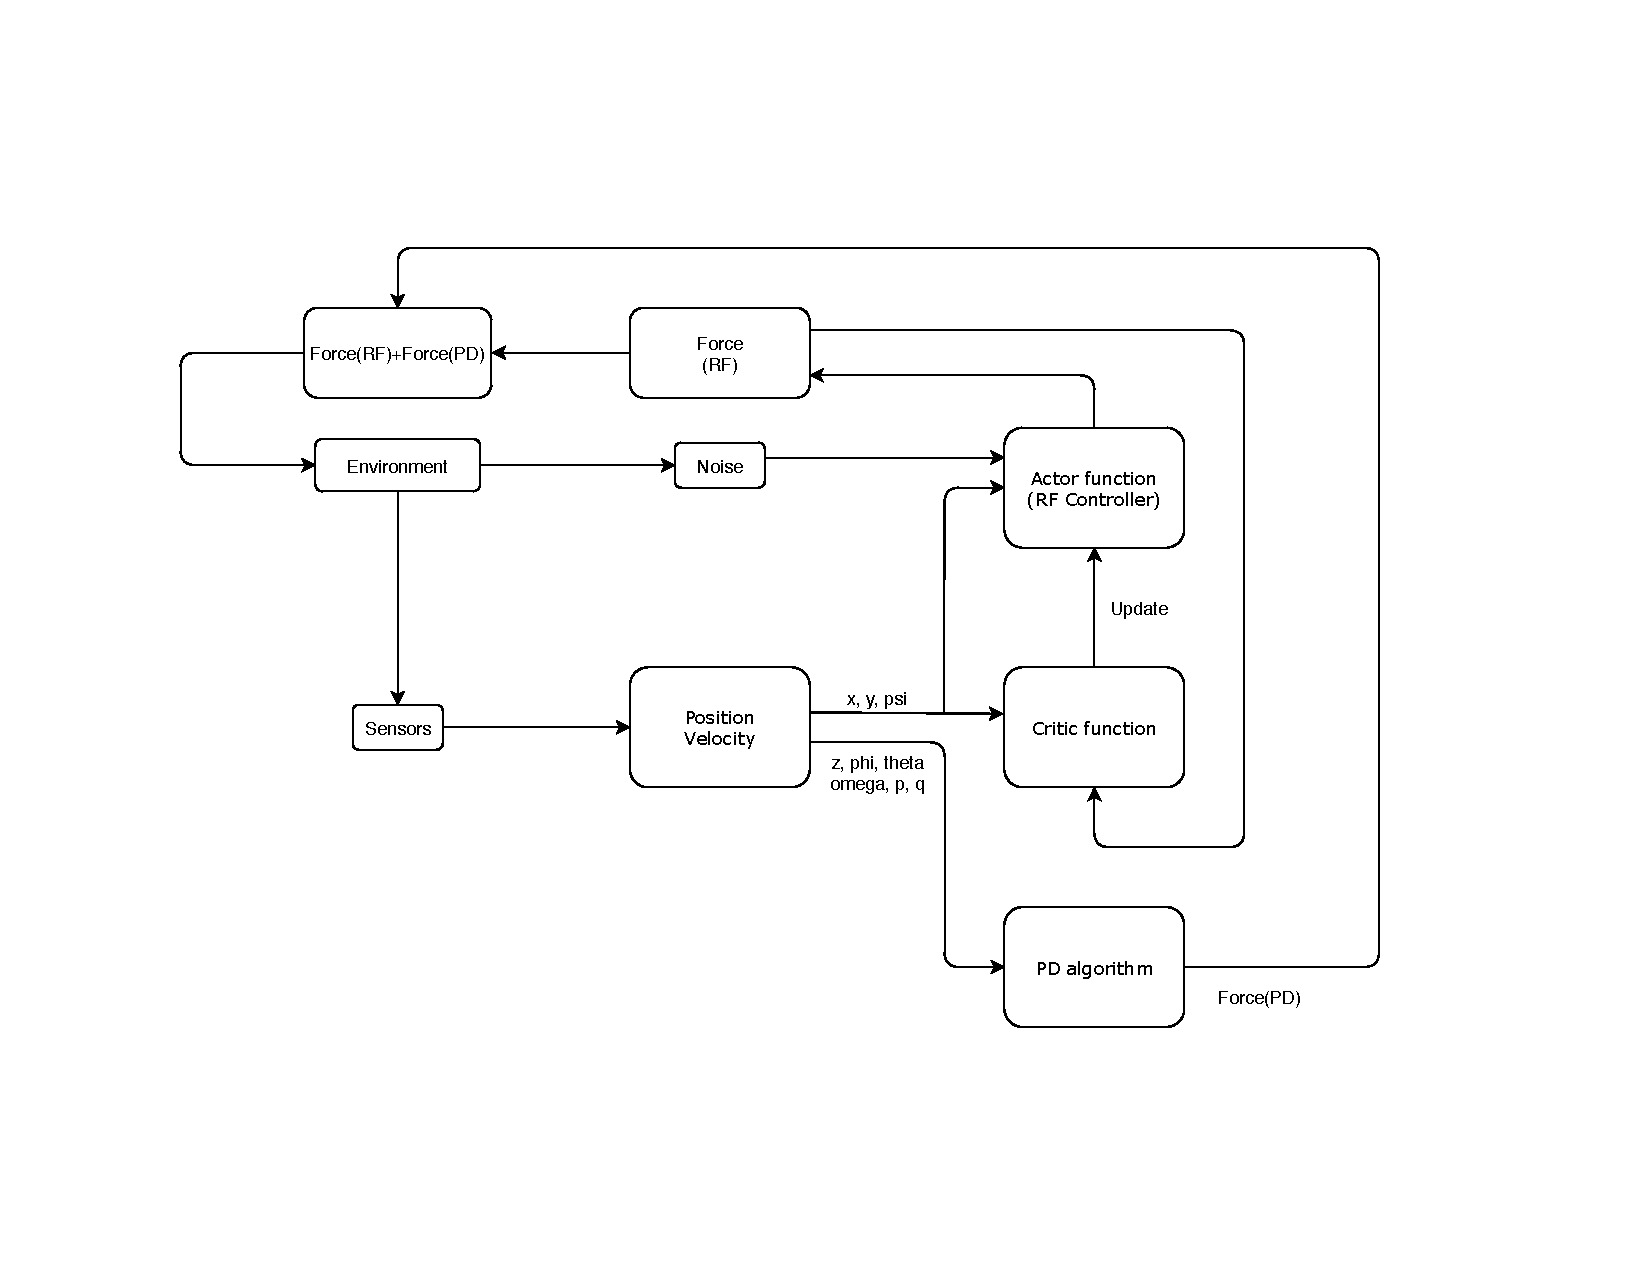
\includegraphics[width=\textwidth, trim={1cm 4cm 1cm 3cm},clip]{images/chap4/architecture.pdf}
    \caption{Controller Architecture for the BlueROV2}
    \label{fig:architecture}
\end{figure}
From the BlueRov2s' sensors the controller receives the pose (position and orientation) and velocities in the given state. The PD algorithm will then receive the pose states $z, \phi, \theta$ and the velocity states $\omega, p, q$, to calculate the needed thrust input in $z, \phi$ and $\theta$. At the same time, the DDPG algorithm will receive the pose states $x, y, \psi$, to calculate the needed thrust input in these states. This results in the thrust input matrix in the given state, $s_{t}$, being equal to
\begin{equation}
    \tau = \begin{bmatrix}
    \tau_{x} \\ \tau_{y} \\ \tau_{z} \\ \tau_{\phi} \\ \tau_{\theta} \\ \tau_{\psi}
    \end{bmatrix}
\end{equation}
The DDPG algorithm is displayed in Algorithm \ref{alg:RF}. As shown in the algorithm, it clips the action ($a_{t}$) based on the constraint $a_{t} \in [-1 , 1]$ and a factor $\epsilon$. $\epsilon$ is here the exploitation versus exploration factor, discussed in chapter \ref{chap:station-keeping}. Both networks also need to be discounted by a \textit{learning rate} $\alpha$, which says something about how much the algorithm values new information in a given state versus the learned optimal actions in that state. The learning rate should also be decreased over the number of iterations, since the algorithm gains larger and lager knowledge about the environment.\\
\begin{algorithm}[H]
\SetAlgoLined
    Initialise the network classes $Q(s_{t},a_{t}|\omega)$ and $\mu(s_{t}|\omega)$ with weights $\omega$ and $\theta$.\\
    Initialise the replay buffer R as a memory class, M, to hold $s_{t}, a_{t}, r_{t}$ and $s_{t+1}$.\\
    \For{ep \textbf{in} MAX\_EPISODES}{
    Initialise episode reward to zero\\
    Initialise episode step, $t$, to zero\\
    \While{t $<$ MAX\_EP\_STEPS}{
    Initialise desired state, $s_{d}$\\
    Initialise desired state PID, $s_{d,PD}$\\
    get position states, $x, y, z$, and orientation states, $\epsilon_{1}, \epsilon_{2}, \epsilon_{3}, \eta$\\
    get the Euler angles $\phi, \theta, \psi$ from the orientation states\\
    compute $s_{t}=(x, y, \psi)$\\
    Choose action $a_{t}=\mu(s_{t}|\theta)$\\
    clip action based on $a_{max}, a_{min}$ and $\epsilon$\\
    compute the error state, $s_{e}$\\
    compute the error state PID, $s_{e, PID}$\\
    compute $r(s_{t},a_{t})$\\
    episode reward += $r(s_{t},a_{t})$\\
    store in transition $R(s_{t},a_{t},r_{t},s_{t+1})$\\
    Randomly select N arrays from R\\
    compute $y_{i}=r_{i}+\gamma Q(s_{i},a_{i}|\omega)$\\
    compute $Loss=\frac{1}{N}\sum_{i=1}^{N}(y_{i}-Q(s_{i},a_{i}|\omega))^{2}$\\
    compute $\nabla_{\omega}Loss=\frac{1}{N}\sum_{i=1}^{N}(y_{i}-Q(s_{i},a_{i}|\omega))\frac{\partial Q(s_{i},a_{i}|\omega)}{\partial \omega}$\\
    update weight $\omega_{t+1}=\omega_{t}+\alpha\nabla_{\omega}Loss$\\
    compute $\nabla_{\theta}J=\frac{1}{N}\sum_{i=1}^{N}\frac{\partial Q(s_{i},a_{i}|\mu(s_{i}|\theta))}{\partial a_{i}}\frac{\partial \mu(s_{i}|\theta)}{\partial\theta}$\\
    compute $m_{t}=\wp\times m_{t-1}+(1-\wp)\nabla_{\theta}\mu$\\
    compute $\Im_{t} & = \beta\times\Im_{t-1}+(1-\beta)\nabla_{\theta}\mu$\\
    compute $\Hat{m}_{t} & = \frac{m_{t}}{1-\wp^{t}}$\\
    compute $\Hat{\Im}_{t} & = \frac{\Im_{t}}{1-\beta^{t}}$\\
    update weight $\theta_{t+1} & = \theta_{t} - \eta\frac{1}{\sqrt{\Hat{\Im}_{t}}}\Hat{m}_{t}$\\
    update weight $\omega^{'}=\rho\omega+(1-\rho)\omega^{'}$ ($\rho$ is learning rate)\\
    update weight $\theta^{'}=\rho\theta+(1-\rho)\theta^{'}$\\
    Get velocity states $[\omega_{t}, p_{t}, q_{t}$]\\
    Get $\tau_{PID}$ from velocity states and $s_{t,PD} = [z, \phi, \theta]$\\
    Set the output thrust equal to: $\tau[0,1,5]=a_{t}$ and $\tau[2,3,4]=\tau_{PD}$\\
    }
    }
\caption{DDPG algorithm}
\label{alg:RF}
\end{algorithm}

\subsection{Reward function}
Optimal design of the reward function, $r(s_{t},a_{t})$, in algorithm \ref{alg:RF} is essential for the behaviour of the algorithm. As mentioned throughout this report, the reward is a feedback from the environment, based on how good it was to take a particular action in a given state. The agent is continuously looking for the highest total cumulative reward, in order to determine the optimal policy starting in any state. Because of this, different reward function designs have been tested, more about this in the next chapter. 
\section{Software}
In order to evaluate the controller design the simulators \textbf{Gazebo} and \textbf{Robotic Operating System} (ROS) were used. Gazebo, which offers the ability to accurately and efficiently simulate a robotic system in complex environments, was used to simulate the \textit{MC Lab} at \textit{Marin Teknisk Senter} in Trondheim, Norway. ROS was used to simulate the dynamics of the \textbf{BlueROV2}, and combining these two resulted in the simulator in figure \ref{fig:ros}. 
\begin{figure}[H]
    \centering
    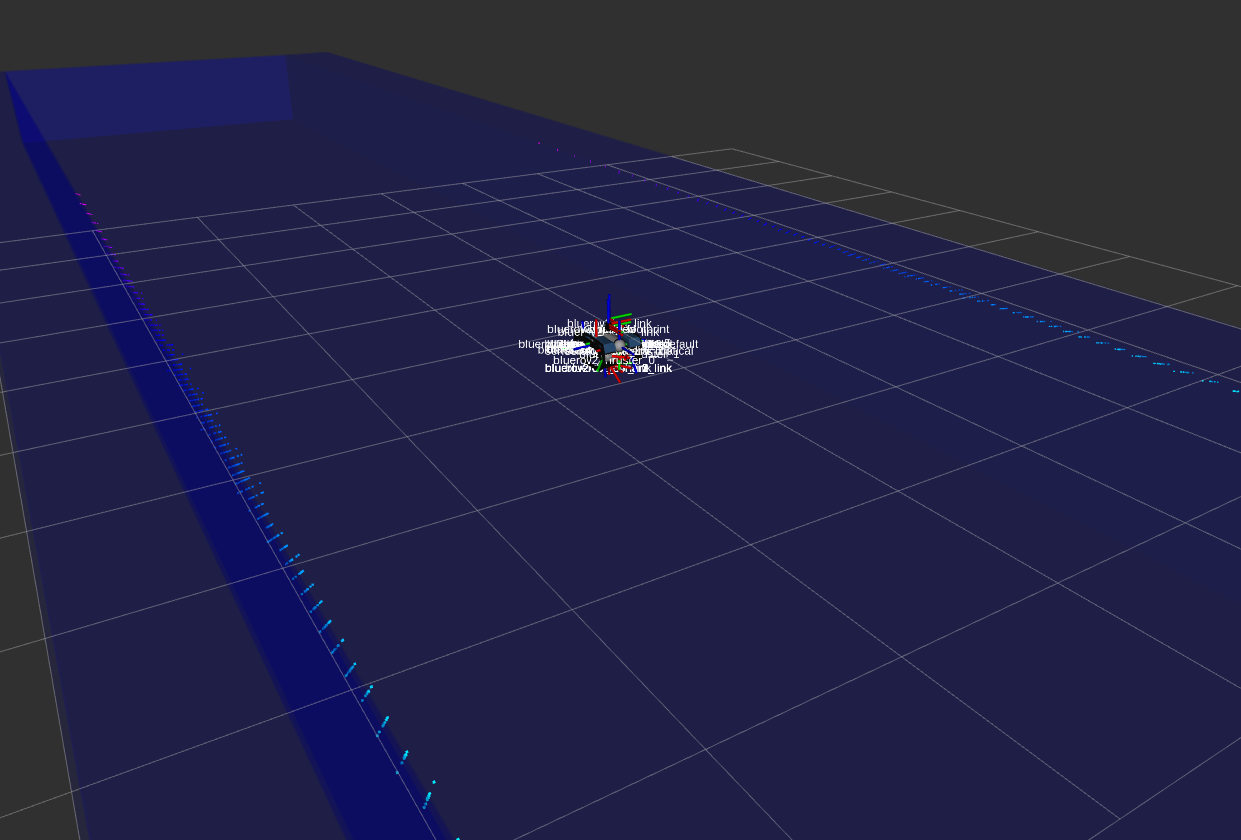
\includegraphics[width=0.7\textwidth]{images/chap4/ROS.png}
    \caption{Gazebo and Robotic Operating System (ROS) with the BlueROV2 AUV}
    \label{fig:ros}
\end{figure}
For the implementation of the controller design, both the DP algorithm and the DDPG algorithm, the programming framework \textit{TensorFlow} was chosen. TensorFlow is an open-source machine learning framework, which works well in combination with the \textit{Python} programming language. 
